
The rest of the analyses all require at least 2 leptons in the final state.
The first analysis in this category is a search for SUSY in a final state with two same sign leptons.
This analysis is an inclusive search designed to be sensitive to many SUSY scenarios.
The baseline selection requires at least two same sign leptons with \pt\ $>$ 10-15 GeV depending on the trigger.

\begin{figure}[!htb]
\begin{center}
\begin{tabular}{cc}
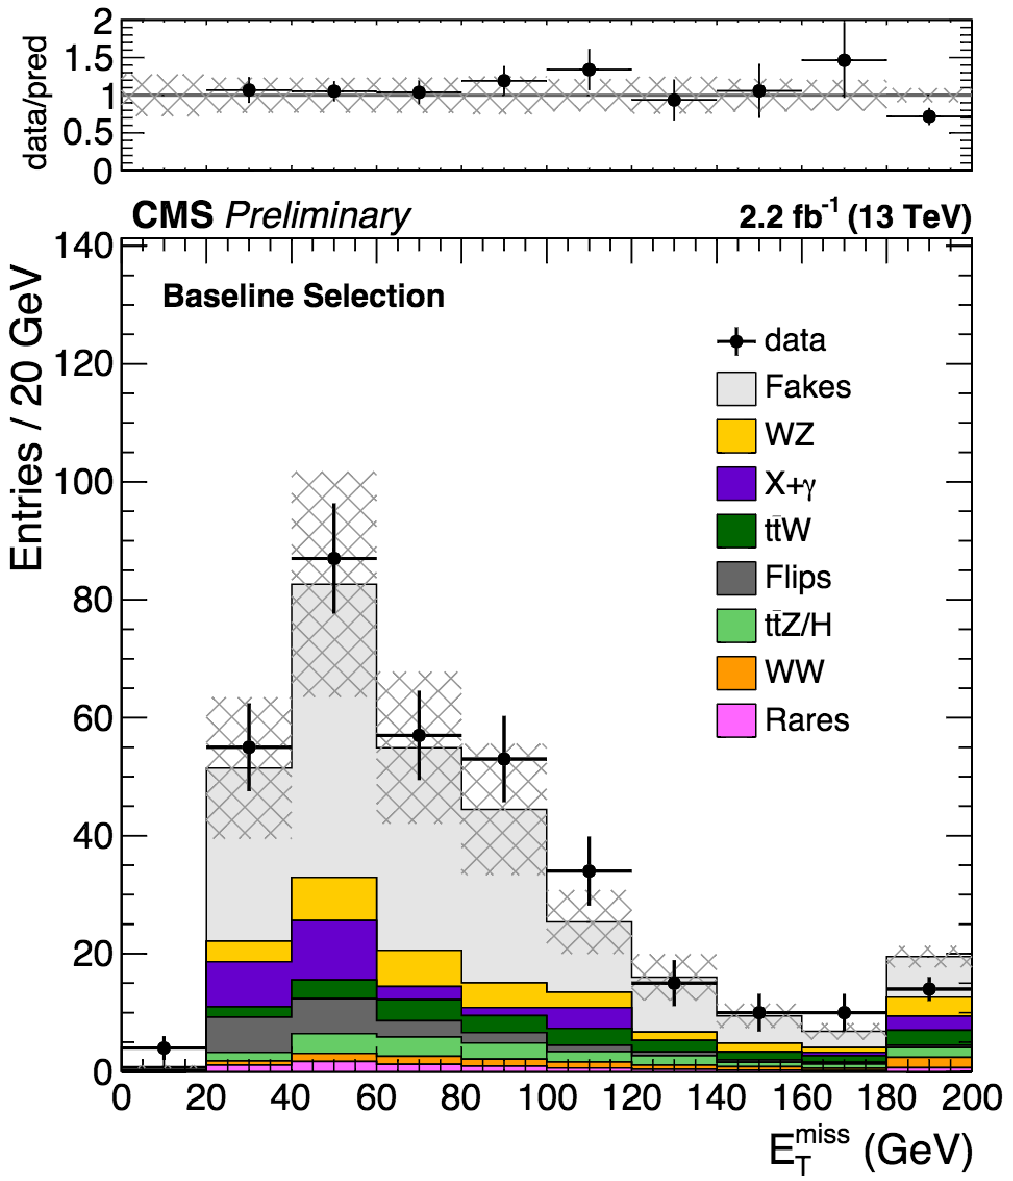
\includegraphics[width=0.4\textwidth]{2lepss/SS_MET.pdf} &
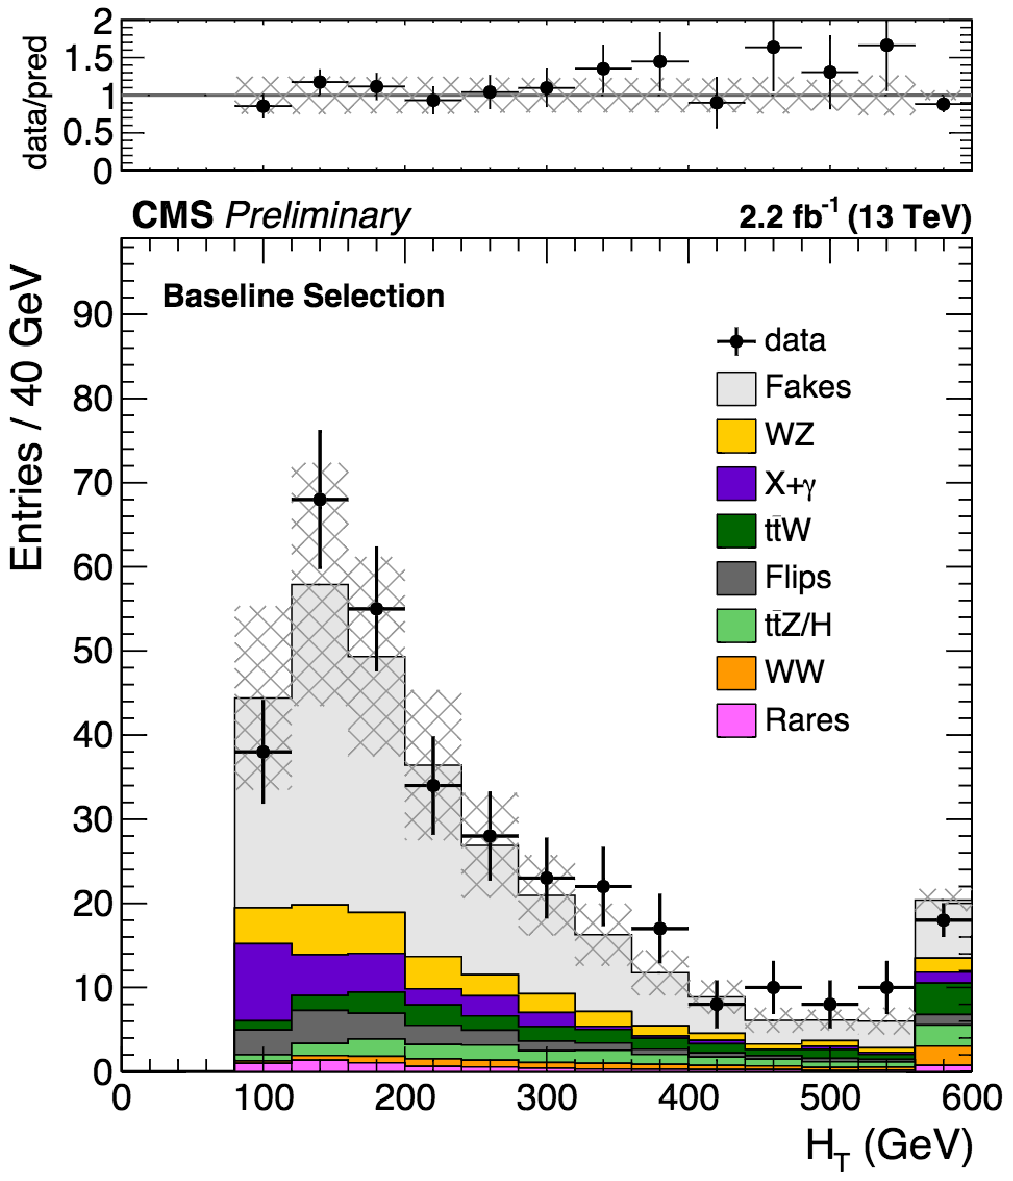
\includegraphics[width=0.4\textwidth]{2lepss/SS_HT.pdf}
\end{tabular}
\caption{
\label{fig:2lepssresults}
Observed yields and background predictions are shown for the same-sign dilepton analysis
for the variables \MET\ (left) and \HT\ (right).
}
\end{center}
\end{figure}


The next analysis is a search in events with three or more leptons.

The final analysis is a search in final states with at least two opposite-sign same-flavor leptons.
In this final state, two separate excesses were seen in run I.
CMS saw an excess in events with Mll 20-70 GeV with a significance of 2.6 sigma where ATLAS saw no excess,
and ATLAS observed a 3 sigma excess in events with two leptons with Mll 81-101, at least large HT, and large MET,
and the result from CMS in a similar signal region showed no significant deviation from the SM prediction.
